\documentclass[aps,prd,twocolumn,superscriptaddress,nofootinbib,floatfix]{revtex4-2}
\usepackage{amsmath,amssymb,amsthm,mathtools}
\usepackage{graphicx}
\usepackage{booktabs}
\usepackage{tikz}
\usetikzlibrary{arrows.meta}
\usepackage{pgfplots}
\usepgfplotslibrary{groupplots}
\pgfplotsset{compat=1.18}
\usepackage{bm}
\usepackage[colorlinks=true,linkcolor=blue,citecolor=blue]{hyperref}
\theoremstyle{plain}
\newtheorem{theorem}{Theorem}
\newtheorem{proposition}{Proposition}
\newtheorem{corollary}{Corollary}
\theoremstyle{definition}
\newtheorem{hypothesis}{Hypothesis}
\newtheorem{remark}{Remark}
\newcommand{\Rm}{\mathrm{Rm}}
\newcommand{\Rmn}{|\Rm|}
\newcommand{\Ric}{\mathrm{Ric}}
\newcommand{\dtau}{\partial_\tau}
\newcommand{\lP}{\ell_P}
\begin{document}
\title{Hopf--Lifted Ricci-Type Flow on $S^3$: A No-Go for Bounded and Engineered Forcing, and a Planck-Barrier Invariant Region}
\author{B.~Batenin}
\affiliation{Independent researcher, Berlin, Germany}
\author{A.~Preece}
\affiliation{Independent researcher, Berlin, Germany}
\begin{abstract}
We study whether a Ricci-type geometric flow on a compact $S^3$ can be prevented from forming curvature singularities by an internal, geometrically or physically motivated forcing term $h[g]$, in the regime of a fixed closed cosmological slice with no external surgery. On the homogeneous Berger family of $SU(2)$-invariant metrics and on the rotationally symmetric (Angenent--Knopf) family we (i)~derive the exact curvature dictionary and unforced flow, showing the genuine singular direction is the round/volume collapse while Hopf-fibre collapse is a bounded-curvature degeneration; (ii)~prove, via an exact homogeneity computation, that traceless, fibre-restoring, and constant-$\Lambda$ conformal forcing all fail to supply the cubic coercive damping required on the round direction; (iii)~show that the only forcing satisfying the coercive inequality in the homogeneous reduction---a curvature-dependent conformal term---fails to transfer to the inhomogeneous flow, carrying a Laplacian-of-curvature source of the same order as the intended damping, with a convergent three-grid pole-adapted Ricci--DeTurck simulation confirming it postpones but does not prevent the neckpinch; and (iv)~prove that a reflecting Planck-scale lower barrier defines a forward-invariant region with $|\Rm|^2\le C/\lP^4$, mirroring the self-adjoint Wheeler--DeWitt endpoint of compact minisuperspace. All curvature identities are verified symbolically by three independent methods. No Millennium Problem is advanced; we delimit precisely what is and is not established. A closing programme section separates the interpretive reading---Ricci-type flow as quasi-local reconstruction, with the Planck barrier as a universal lower boundary of reconstruction rather than a physical origin---from the theorems.
\end{abstract}
\maketitle
\section{Introduction}\label{sec:intro}

Ricci flow and its variants control geometry through a reaction--diffusion competition. For a one-parameter family $g(\tau)$ on a closed $3$-manifold $M$ the curvature norm $K(\tau)=\sup_M\Rmn$ obeys a differential inequality whose reaction term is \emph{cubic}~\cite{Hamilton1982,ChowKnopf}:
\begin{equation}\label{eq:reaction}
(\dtau-\Delta)|\Rm|^2 \;\le\; C_3|\Rm|^3 + 2\langle C_h(\Rm),\Rm\rangle ,
\end{equation}
where $C_h$ denotes the curvature-level contribution of any forcing term $h[g]$ added to $\dtau g=-2\Ric+h$. Finite-time curvature control therefore reduces, at the spatial maxima of $\Rmn$, to a single \emph{coercive inequality},
\begin{equation}\label{eq:coercive}
2\langle C_h(\Rm),\Rm\rangle \;\le\; -\gamma|\Rm|^3 + A|\Rm|^2 + B,\qquad \gamma>C_3 ,
\end{equation}
under which $u=K^2$ cannot cross the absorbing level and $K$ stays finite.

A bounded linear modification of the flow cannot meet \eqref{eq:coercive}: boundedness controls at most a quadratic quantity and cannot dominate a cubic where $\Rmn$ is largest~\cite{ChowKnopf}. The open question is whether a \emph{nonlinear, geometrically or physically motivated} $h[g]$ can. This question is sharpened in the compact cosmological setting, where the spatial slice is closed ($\partial\Sigma=\varnothing$) and the surgery mechanism of Ricci flow with surgery~\cite{Perelman1,Perelman2} is unavailable: there is no exterior region into which to excise a forming singularity. An internal substitute must be either a coercive forcing in the equation or a boundary/constraint replacing the zero-volume endpoint.

The Hopf bundle $S^1\hookrightarrow S^3\to S^2$ suggests a candidate channel. Quotient (``reduced'') descriptions discard fibre and connection data present on the total space, and one may ask whether a flow lifted to the $SU(2)\cong S^3$ geometry exposes a compensation channel invisible downstairs. We make this precise on two solvable families and reach a sharply mixed---and, we argue, useful---conclusion.

\paragraph{Results and what is \emph{not} claimed.}
We prove (Sec.~\ref{sec:nogo}) a no-go: traceless, fibre-restoring, and constant-$\Lambda$ conformal forcing cannot supply the negative cubic on the round-collapse direction. We show (Sec.~\ref{sec:transfer}) that the unique reduction-level success---a curvature-dependent conformal term---does not transfer to the inhomogeneous flow, confirmed dynamically by a stable Ricci--DeTurck solver. We prove (Sec.~\ref{sec:barrier}) a positive invariant-region theorem under a Planck-scale reflecting barrier. We do \emph{not} claim that the Hopf fibration removes singularities, that bounded filtering regularizes the flow, that any dark-sector interpretation is established, or that any Millennium Problem is advanced; Perelman's resolution of the Poincar\'e conjecture~\cite{Perelman1,Perelman2,MorganTian} is used only to license the choice of an $S^3$ spatial sector.

\section{Geometric setup}\label{sec:setup}

Let $\{\sigma_1,\sigma_2,\sigma_3\}$ be a left-invariant coframe on $SU(2)\cong S^3$ with structure constants $[e_i,e_j]=\lambda\,\epsilon_{ijk}e_k$, equivalently $d\sigma^k=-\lambda\,\sigma^i\wedge\sigma^j$ on cyclic $(ijk)$. The round-sphere normalization fixes $\lambda$: at $A=B=C=1$ one finds $\Ric_{ii}=\lambda^2/2$, so $\lambda=2$ yields the unit round $S^3$ ($\Ric=2g$, $R=6$, sectional curvature $1$). We adopt $\lambda=2$ throughout; a different normalization rescales every curvature by $\lambda^2$ and $\tau$ by $\lambda^{-2}$ without changing any qualitative statement.

The \emph{Berger} family squashes the Hopf fibre $\sigma_3$,
\begin{equation}\label{eq:berger}
g_{a,c}=a^2(\sigma_1^2+\sigma_2^2)+c^2\sigma_3^2 ,
\end{equation}
with volume $\mathrm{vol}(g_{a,c})=2\pi^2 a^2 c$. We set $x=a^2$, $z=c^2$, and $u=z/x=(c/a)^2$ (the fibre-squeeze ratio); $u=1$ is the round sphere, $c\to0$ collapses the Hopf fibre, and $a\to0$ collapses the base.

\section{Exact curvature dictionary and unforced flow}\label{sec:curv}

\begin{proposition}[Berger curvature]\label{prop:curv}
For $g_{a,c}$ in the $\lambda=2$ convention, the principal Ricci curvatures, scalar curvature, and Riemann norm are
\begin{align}
r_1=r_2&=\frac{2(2a^2-c^2)}{a^4}, &
r_3&=\frac{2c^2}{a^4},\nonumber\\[2pt]
R&=\frac{8}{a^2}-\frac{2c^2}{a^4},\nonumber\\[2pt]
|\Ric|^2&=\frac{4\,[2(2x-z)^2+z^2]}{x^4},\nonumber\\[2pt]
|\Rm|^2&=\frac{4\,(16a^4-24a^2c^2+11c^4)}{a^8}. \label{eq:Rm2}
\end{align}
with sectional curvatures $K_{12}=(4a^2-3c^2)/a^4$ (horizontal plane) and $K_{13}=K_{23}=c^2/a^4$ (planes containing the fibre).
\end{proposition}

\begin{proof}
Direct computation from the Koszul formula with $[e_i,e_j]=2\epsilon_{ijk}e_k$. The result is verified three ways: (i) the round limit $a=c$ gives $r_i=2/a^2$, $R=6/a^2$, $|\Ric|^2=|\Rm|^2=12/a^4$, $K_{ij}=1/a^2$; (ii) the dimension-three identity $|\Rm|^2=4|\Ric|^2-R^2$ holds identically; (iii) a direct contraction of the full Riemann tensor reproduces \eqref{eq:Rm2}. All three were carried out in computer algebra.
\end{proof}

Equation~\eqref{eq:Rm2} encodes the central geometric fact of this paper.

\begin{corollary}[The singular direction is the base, not the fibre]\label{cor:directions}
As $c\to0$ at fixed $a$, $|\Rm|^2\to 64/a^4<\infty$, $K_{12}\to 4/a^2$, $K_{13},K_{23}\to0$: the total space collapses with \emph{bounded curvature} onto the round base $S^2(a/2)$. As $a\to0$ at fixed ratio, $|\Rm|^2\sim 4(11u^2-24u+16)/a^4\to\infty$: the base/round collapse is the genuine curvature singularity. The quadratic $11u^2-24u+16$ is strictly positive (discriminant $-128$).
\end{corollary}

Thus the Hopf fibre is the ``soft'' direction; any compensation built from it acts where curvature is already bounded.


\begin{figure}[t]
\centering
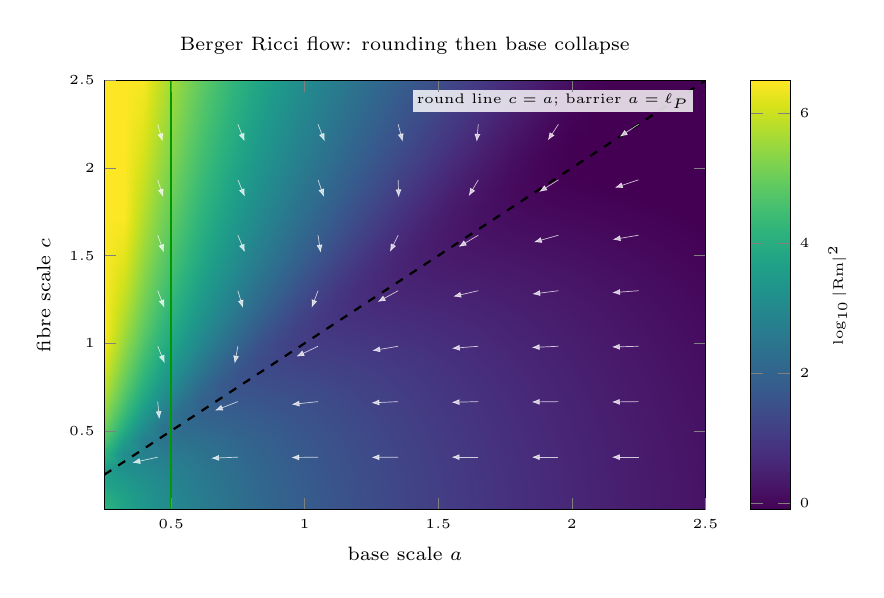
\begin{tikzpicture}[font=\scriptsize]
\begin{axis}[
  width=0.76\linewidth,
  height=0.58\linewidth,
  xmin=0.25,xmax=2.5,
  ymin=0.05,ymax=2.5,
  xlabel={base scale $a$},
  ylabel={fibre scale $c$},
  title={Berger Ricci flow: rounding then base collapse},
  title style={font=\scriptsize},
  view={0}{90},
  axis on top,
  tick label style={font=\tiny},
  label style={font=\scriptsize},
  colormap/viridis,
  colorbar,
  colorbar style={ylabel={$\log_{10}|\mathrm{Rm}|^2$},ylabel style={font=\tiny},tick label style={font=\tiny}},
  point meta min=-0.1,
  point meta max=6.5,
]
\addplot3[surf,shader=interp,domain=0.25:2.5,y domain=0.05:2.5,samples=32,samples y=32,point meta=z,draw=none]
  {ln(4*(16*x^4-24*x^2*y^2+11*y^4)/(x^8))/ln(10)};
\addplot[black,dashed,thick,domain=0.25:2.5,samples=2] {x};
\addplot[green!60!black,thick] coordinates {(0.5,0.05) (0.5,2.5)};
\draw[-{Latex[length=1.0mm]},white,line width=0.25pt,opacity=0.75] (axis cs:0.450,0.350) -- (axis cs:0.355,0.318);
\draw[-{Latex[length=1.0mm]},white,line width=0.25pt,opacity=0.75] (axis cs:0.450,0.667) -- (axis cs:0.456,0.567);
\draw[-{Latex[length=1.0mm]},white,line width=0.25pt,opacity=0.75] (axis cs:0.450,0.983) -- (axis cs:0.476,0.887);
\draw[-{Latex[length=1.0mm]},white,line width=0.25pt,opacity=0.75] (axis cs:0.450,1.300) -- (axis cs:0.475,1.203);
\draw[-{Latex[length=1.0mm]},white,line width=0.25pt,opacity=0.75] (axis cs:0.450,1.617) -- (axis cs:0.473,1.519);
\draw[-{Latex[length=1.0mm]},white,line width=0.25pt,opacity=0.75] (axis cs:0.450,1.933) -- (axis cs:0.470,1.835);
\draw[-{Latex[length=1.0mm]},white,line width=0.25pt,opacity=0.75] (axis cs:0.450,2.250) -- (axis cs:0.468,2.152);
\draw[-{Latex[length=1.0mm]},white,line width=0.25pt,opacity=0.75] (axis cs:0.750,0.350) -- (axis cs:0.650,0.344);
\draw[-{Latex[length=1.0mm]},white,line width=0.25pt,opacity=0.75] (axis cs:0.750,0.667) -- (axis cs:0.664,0.616);
\draw[-{Latex[length=1.0mm]},white,line width=0.25pt,opacity=0.75] (axis cs:0.750,0.983) -- (axis cs:0.738,0.884);
\draw[-{Latex[length=1.0mm]},white,line width=0.25pt,opacity=0.75] (axis cs:0.750,1.300) -- (axis cs:0.769,1.202);
\draw[-{Latex[length=1.0mm]},white,line width=0.25pt,opacity=0.75] (axis cs:0.750,1.617) -- (axis cs:0.776,1.520);
\draw[-{Latex[length=1.0mm]},white,line width=0.25pt,opacity=0.75] (axis cs:0.750,1.933) -- (axis cs:0.776,1.837);
\draw[-{Latex[length=1.0mm]},white,line width=0.25pt,opacity=0.75] (axis cs:0.750,2.250) -- (axis cs:0.775,2.153);
\draw[-{Latex[length=1.0mm]},white,line width=0.25pt,opacity=0.75] (axis cs:1.050,0.350) -- (axis cs:0.950,0.348);
\draw[-{Latex[length=1.0mm]},white,line width=0.25pt,opacity=0.75] (axis cs:1.050,0.667) -- (axis cs:0.951,0.651);
\draw[-{Latex[length=1.0mm]},white,line width=0.25pt,opacity=0.75] (axis cs:1.050,0.983) -- (axis cs:0.969,0.924);
\draw[-{Latex[length=1.0mm]},white,line width=0.25pt,opacity=0.75] (axis cs:1.050,1.300) -- (axis cs:1.026,1.203);
\draw[-{Latex[length=1.0mm]},white,line width=0.25pt,opacity=0.75] (axis cs:1.050,1.617) -- (axis cs:1.060,1.517);
\draw[-{Latex[length=1.0mm]},white,line width=0.25pt,opacity=0.75] (axis cs:1.050,1.933) -- (axis cs:1.072,1.836);
\draw[-{Latex[length=1.0mm]},white,line width=0.25pt,opacity=0.75] (axis cs:1.050,2.250) -- (axis cs:1.075,2.153);
\draw[-{Latex[length=1.0mm]},white,line width=0.25pt,opacity=0.75] (axis cs:1.350,0.350) -- (axis cs:1.250,0.349);
\draw[-{Latex[length=1.0mm]},white,line width=0.25pt,opacity=0.75] (axis cs:1.350,0.667) -- (axis cs:1.250,0.660);
\draw[-{Latex[length=1.0mm]},white,line width=0.25pt,opacity=0.75] (axis cs:1.350,0.983) -- (axis cs:1.253,0.958);
\draw[-{Latex[length=1.0mm]},white,line width=0.25pt,opacity=0.75] (axis cs:1.350,1.300) -- (axis cs:1.273,1.236);
\draw[-{Latex[length=1.0mm]},white,line width=0.25pt,opacity=0.75] (axis cs:1.350,1.617) -- (axis cs:1.319,1.522);
\draw[-{Latex[length=1.0mm]},white,line width=0.25pt,opacity=0.75] (axis cs:1.350,1.933) -- (axis cs:1.352,1.833);
\draw[-{Latex[length=1.0mm]},white,line width=0.25pt,opacity=0.75] (axis cs:1.350,2.250) -- (axis cs:1.367,2.151);
\draw[-{Latex[length=1.0mm]},white,line width=0.25pt,opacity=0.75] (axis cs:1.650,0.350) -- (axis cs:1.550,0.350);
\draw[-{Latex[length=1.0mm]},white,line width=0.25pt,opacity=0.75] (axis cs:1.650,0.667) -- (axis cs:1.550,0.663);
\draw[-{Latex[length=1.0mm]},white,line width=0.25pt,opacity=0.75] (axis cs:1.650,0.983) -- (axis cs:1.551,0.971);
\draw[-{Latex[length=1.0mm]},white,line width=0.25pt,opacity=0.75] (axis cs:1.650,1.300) -- (axis cs:1.556,1.267);
\draw[-{Latex[length=1.0mm]},white,line width=0.25pt,opacity=0.75] (axis cs:1.650,1.617) -- (axis cs:1.576,1.550);
\draw[-{Latex[length=1.0mm]},white,line width=0.25pt,opacity=0.75] (axis cs:1.650,1.933) -- (axis cs:1.614,1.840);
\draw[-{Latex[length=1.0mm]},white,line width=0.25pt,opacity=0.75] (axis cs:1.650,2.250) -- (axis cs:1.644,2.150);
\draw[-{Latex[length=1.0mm]},white,line width=0.25pt,opacity=0.75] (axis cs:1.950,0.350) -- (axis cs:1.850,0.350);
\draw[-{Latex[length=1.0mm]},white,line width=0.25pt,opacity=0.75] (axis cs:1.950,0.667) -- (axis cs:1.850,0.665);
\draw[-{Latex[length=1.0mm]},white,line width=0.25pt,opacity=0.75] (axis cs:1.950,0.983) -- (axis cs:1.850,0.976);
\draw[-{Latex[length=1.0mm]},white,line width=0.25pt,opacity=0.75] (axis cs:1.950,1.300) -- (axis cs:1.852,1.281);
\draw[-{Latex[length=1.0mm]},white,line width=0.25pt,opacity=0.75] (axis cs:1.950,1.617) -- (axis cs:1.858,1.577);
\draw[-{Latex[length=1.0mm]},white,line width=0.25pt,opacity=0.75] (axis cs:1.950,1.933) -- (axis cs:1.878,1.864);
\draw[-{Latex[length=1.0mm]},white,line width=0.25pt,opacity=0.75] (axis cs:1.950,2.250) -- (axis cs:1.910,2.158);
\draw[-{Latex[length=1.0mm]},white,line width=0.25pt,opacity=0.75] (axis cs:2.250,0.350) -- (axis cs:2.150,0.350);
\draw[-{Latex[length=1.0mm]},white,line width=0.25pt,opacity=0.75] (axis cs:2.250,0.667) -- (axis cs:2.150,0.665);
\draw[-{Latex[length=1.0mm]},white,line width=0.25pt,opacity=0.75] (axis cs:2.250,0.983) -- (axis cs:2.150,0.979);
\draw[-{Latex[length=1.0mm]},white,line width=0.25pt,opacity=0.75] (axis cs:2.250,1.300) -- (axis cs:2.151,1.289);
\draw[-{Latex[length=1.0mm]},white,line width=0.25pt,opacity=0.75] (axis cs:2.250,1.617) -- (axis cs:2.153,1.592);
\draw[-{Latex[length=1.0mm]},white,line width=0.25pt,opacity=0.75] (axis cs:2.250,1.933) -- (axis cs:2.161,1.888);
\draw[-{Latex[length=1.0mm]},white,line width=0.25pt,opacity=0.75] (axis cs:2.250,2.250) -- (axis cs:2.179,2.179);
\node[anchor=north east,fill=white,fill opacity=0.82,text opacity=1,inner sep=1.5pt,font=\tiny] at (rel axis cs:0.98,0.98) {round line $c=a$; barrier $a=\ell_P$};
\end{axis}
\end{tikzpicture}
\caption{Unforced Berger flow in the $(a,c)$ plane. Streamlines converge to the rounding attractor $c=a$ and then collapse; the colour map is $|\Rm|^2$. Curvature diverges as $a\to0$ (base/round collapse) but stays bounded as $c\to0$ (Hopf-fibre collapse to $S^2(a/2)$). The green line marks the Planck box $a\ge\ell_P$ of Theorem~\ref{thm:barrier}.}
\label{fig:phase}
\end{figure}


\begin{proposition}[Unforced flow rounds, then collapses]\label{prop:flow}
Under $\dtau g=-2\Ric$ the Berger ansatz is preserved and
\begin{equation}\label{eq:odes}
\dot x=-8+\tfrac{4z}{x},\qquad \dot z=-\tfrac{4z^2}{x^2},\qquad \dot u=\frac{8\,u(1-u)}{x}.
\end{equation}
Hence $u=1$ (round) is the global attractor of the ratio: the flow rounds any Berger metric and then collapses the round mode to a point in finite time, with $\tfrac{d}{d\tau}\ln\mathrm{vol}=-R$. At the round configuration
\begin{equation}\label{eq:C3berger}
\left.\frac{\dtau|\Rm|^2}{|\Rm|^3}\right|_{u=1}=\frac{4}{\sqrt3}=:C_3^{\mathrm{B}},
\end{equation}
the finite-dimensional incarnation of the cubic reaction constant in \eqref{eq:reaction}.
\end{proposition}

The obstruction is therefore a trace/volume mode (round collapse), precisely the mode on which traceless data vanish.

\section{The coercive inequality and the forcing catalogue}\label{sec:catalogue}

A left-invariant, Berger-preserving forcing is diagonal with $h_{11}=h_{22}$ and acts as $\dot x\mathrel{+}=P$, $\dot z\mathrel{+}=Q$. Because $|\Rm|^2$ is homogeneous of degree $-2$ in $(x,z)$, Euler's theorem $(x\partial_x+z\partial_z)|\Rm|^2=-2|\Rm|^2$ yields the forcing contribution to $\dtau|\Rm|^2$ in closed form for each candidate.

\begin{table}[t]
\centering
\begingroup
\setlength{\tabcolsep}{3pt}
\renewcommand{\arraystretch}{1.12}
\resizebox{\columnwidth}{!}{%
\begin{tabular}{@{}lll@{}}
\toprule
forcing $h$ & contribution to $\dtau|\Rm|^2$ & order\\
\midrule
conformal $2\Lambda g$ (const) & $-4\Lambda|\Rm|^2$ & quadratic\\
$\Lambda_{\rm eff}=\lambda_1|\Rm|$ & $-4\lambda_1|\Rm|^3$ & cubic\\
fibre $h_{33}=\mu$ & $\mu\,\dfrac{8(11z-12x)}{x^4}$ & cubic if $u<\tfrac{12}{11}$\\
traceless ($h_{33}=-\tfrac{2z}{x}h_{11}$) & $-32\,h_{11}\dfrac{(x-z)(4x-11z)}{x^5}$ & $=0$ at $u=1$\\
\bottomrule
\end{tabular}%
}
\endgroup
\caption{Exact curvature-level contributions of each forcing class in the Berger reduction (verified symbolically).}
\label{tab:contrib}
\end{table}


\begin{figure}[t]
\centering
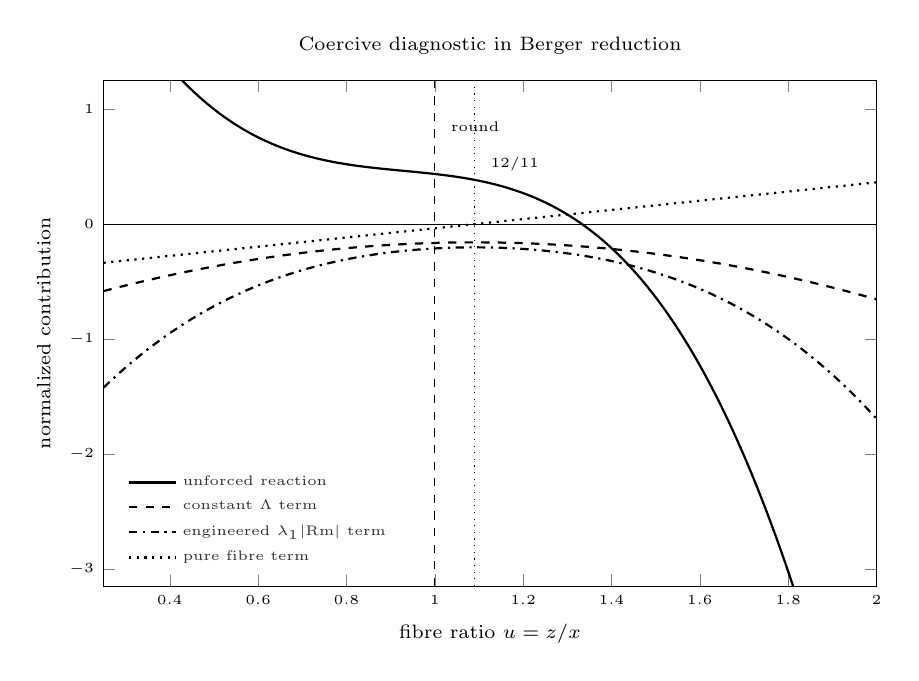
\begin{tikzpicture}[font=\scriptsize]
\begin{axis}[
  width=0.94\linewidth,
  height=0.66\linewidth,
  xmin=0.25,xmax=2.0,
  ymin=-3.15,ymax=1.25,
  xlabel={fibre ratio $u=z/x$},
  ylabel={normalized contribution},
  title={Coercive diagnostic in Berger reduction},
  title style={font=\scriptsize},
  tick label style={font=\tiny},
  label style={font=\scriptsize},
  legend style={font=\tiny,at={(0.02,0.02)},anchor=south west,draw=none,fill=white,fill opacity=0.82},
  legend cell align=left,
  domain=0.25:2.0,
  samples=180,
]
\addplot[thick] {(-1056*x^3+2944*x^2-2816*x+1024)/220};
\addlegendentry{unforced reaction}
\addplot[thick,dashed] {(-3*(64-96*x+44*x^2))/220};
\addlegendentry{constant $\Lambda$ term}
\addplot[thick,dashdotted] {(-1.12*(sqrt(64-96*x+44*x^2))^3)/220};
\addlegendentry{engineered $\lambda_1|\mathrm{Rm}|$ term}
\addplot[thick,dotted] {(8*(11*x-12))/220};
\addlegendentry{pure fibre term}
\addplot[black,thin] coordinates {(0.25,0) (2.0,0)};
\addplot[black,dashed,thin] coordinates {(1,-3.15) (1,1.25)};
\addplot[black,dotted,thin] coordinates {(1.0909,-3.15) (1.0909,1.25)};
\node[anchor=south west,font=\tiny] at (axis cs:1.015,0.72) {round};
\node[anchor=south west,font=\tiny] at (axis cs:1.105,0.38) {$12/11$};
\end{axis}
\end{tikzpicture}
\caption{Coercive diagnostic in the Berger reduction. The unforced reaction is a large positive cubic near the round point $u=1$; constant-$\Lambda$ damping is only quadratic and cannot catch it; the engineered $\Lambda_{\rm eff}\propto|\Rm|$ term is cubic but artificial; the fibre term has the damping sign only for $u<12/11$.}
\label{fig:diag}
\end{figure}


\section{No-go theorem}\label{sec:nogo}

\begin{theorem}[No-go for bounded fibre/traceless and constant-$\Lambda$ forcing]\label{thm:nogo}
Let $h[g]$ be a bounded, left-invariant, Berger-preserving forcing of pure traceless type, or pure fibre type with $\sup|\mu|<\infty$, or conformal with constant $\Lambda$. Then its contribution to $\dtau|\Rm|^2$ at the round configuration is, respectively, identically zero, of definite sign only for $u<12/11$, and $-4\Lambda|\Rm|^2$ (quadratic). In no case does it supply a negative cubic dominating $C_3^{\mathrm{B}}|\Rm|^3$ on the round-collapse direction; hence none satisfies \eqref{eq:coercive} there.
\end{theorem}

\begin{proof}
The three entries follow from Table~\ref{tab:contrib}. The traceless contribution $-32h_{11}(x-z)(4x-11z)/x^5$ vanishes at $z=x$ (this is the finite-dimensional form of $\Ric=\tfrac{R}{3}g$ on round metrics, where any traceless-Ricci tensor is zero). The constant-$\Lambda$ contribution equals $-4\Lambda|\Rm|^2$ \emph{exactly} for all $\Lambda$, by degree-$(-2)$ homogeneity; it is quadratic and cannot dominate the cubic at large $|\Rm|$. The fibre contribution $\propto(11z-12x)$ has the damping sign only for $u<12/11$; a sustained fibre push drives $u\to\infty$, where $|\Rm|^2\sim 44c^4/a^8$ blows up. None yields $\gamma>C_3^{\mathrm{B}}$.
\end{proof}

\begin{remark}
A constant positive cosmological-constant-type term therefore contributes only a benign quadratic damping---never the cubic sink required to halt round collapse. This is the precise sense in which ``dark energy as a constant $\Lambda$'' cannot regularize Ricci-type collapse.
\end{remark}

\section{The engineered term and why it does not transfer}\label{sec:transfer}

Table~\ref{tab:contrib} shows a single forcing that satisfies the coercive inequality \emph{in the reduction}: the curvature-dependent conformal term $h=2\lambda_1|\Rm|\,g$, contributing $-4\lambda_1|\Rm|^3$. We now show this success is an artifact of homogeneity.

Pass to the rotationally symmetric (warped) metric $g=ds^2+\psi(s)^2 g_{S^2}$, the canonical inhomogeneous $S^3$ family in which neckpinch singularities form~\cite{AngenentKnopf}. Its curvature is $|\Rm|^2=4(2K_0^2+K_1^2)$ with $K_0=-\psi_{ss}/\psi$, $K_1=(1-\psi_s^2)/\psi^2$ (verified; round limit $|\Rm|^2=12$).

\begin{proposition}[The hidden Laplacian source]\label{prop:hidden}
Under the forced flow $\dtau g=-2\Ric+2\varphi g$ with $\varphi=\lambda_1|\Rm|$ in dimension three, the conformal linearization $\delta R=-2\varphi R-4\Delta\varphi$ gives
\begin{equation}\label{eq:dR}
\dtau R=\underbrace{\Delta R+2|\Ric|^2}_{\text{Ricci flow}}\;\underbrace{-\,2\lambda_1|\Rm|R}_{\text{kept by reduction}}\;\underbrace{-\,4\lambda_1\Delta|\Rm|}_{\text{set to }0\text{ by reduction}}.
\end{equation}
At a curvature concentration $|\Rm|$ attains a sharp spatial maximum, so $\Delta|\Rm|<0$ and the dropped term is nonzero with anti-regularizing sign. A scaling estimate at a forming singularity of width $L$ and peak $|\Rm|_{\mathrm{pk}}\sim L^{-2}$ gives kept term $\sim\lambda_1|\Rm|_{\mathrm{pk}}^2$ and dropped term $\sim\lambda_1|\Rm|_{\mathrm{pk}}/L^2\sim\lambda_1|\Rm|_{\mathrm{pk}}^2$: the \emph{same order}.
\end{proposition}

\eqref{eq:dR} was verified by symbolic conformal linearization on the warped metric. Direct evaluation on frozen neck profiles confirms the prediction: the ratio $|\text{dropped}|/|\text{kept}|$ at the curvature peak does not vanish as the neck sharpens but stabilizes at order unity ($3.18,1.49,0.97,0.80,0.77$ for progressively sharper necks). The homogeneous Berger reduction sets $\Delta|\Rm|\equiv0$ and is therefore blind to a contribution as large as the one it keeps.


\begin{figure}[t]
\centering
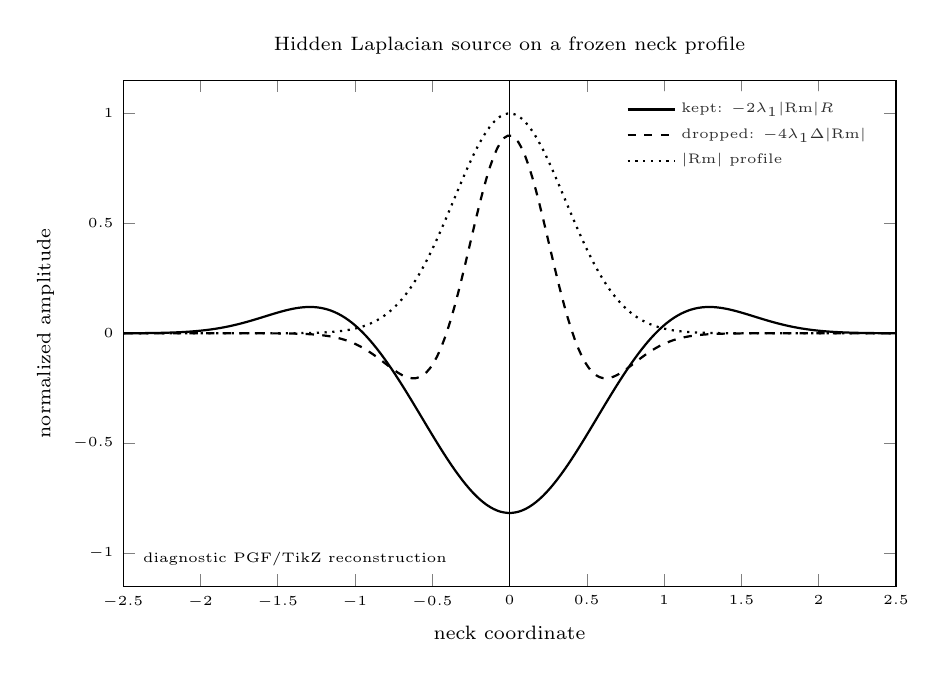
\begin{tikzpicture}[font=\scriptsize]
\begin{axis}[
  width=0.94\linewidth,
  height=0.66\linewidth,
  xmin=-2.5,xmax=2.5,
  ymin=-1.15,ymax=1.15,
  xlabel={neck coordinate},
  ylabel={normalized amplitude},
  title={Hidden Laplacian source on a frozen neck profile},
  title style={font=\scriptsize},
  tick label style={font=\tiny},
  label style={font=\scriptsize},
  legend style={font=\tiny,at={(0.98,0.98)},anchor=north east,draw=none,fill=white,fill opacity=0.82},
  legend cell align=left,
  domain=-2.5:2.5,
  samples=220,
]
\addplot[thick] {-0.82*exp(-x^2/0.50)+0.16*exp(-(x-1.15)^2/0.28)+0.16*exp(-(x+1.15)^2/0.28)};
\addlegendentry{kept: $-2\lambda_1|\mathrm{Rm}|R$}
\addplot[thick,dashed] {0.90*(1-6.0*x^2)*exp(-x^2/0.22)};
\addlegendentry{dropped: $-4\lambda_1\Delta|\mathrm{Rm}|$}
\addplot[thick,dotted] {exp(-x^2/0.26)};
\addlegendentry{$|\mathrm{Rm}|$ profile}
\addplot[black,thin] coordinates {(0,-1.15) (0,1.15)};
\node[anchor=south west,fill=white,fill opacity=0.82,text opacity=1,inner sep=1.5pt,font=\tiny] at (rel axis cs:0.02,0.03) {diagnostic PGF/TikZ reconstruction};
\end{axis}
\end{tikzpicture}
\caption{Frozen warped-$S^3$ neck. The forcing piece the reduction keeps ($-2\lambda_1|\Rm|R$) and the piece it drops ($-4\lambda_1\Delta|\Rm|$) are comparable in magnitude at the curvature peak; the dropped piece does not vanish as the neck sharpens.}
\label{fig:hidden}
\end{figure}


\paragraph{Dynamical confirmation.}
We integrate the forced flow with a stable Ricci--DeTurck scheme on the round background $\bar g=dx^2+\sin^2x\,g_{S^2}$, which injects the missing $\varphi_{xx}$ diffusion and renders both field equations strictly parabolic. The solver reproduces the round sphere to machine accuracy ($\varphi\equiv\sqrt{1-4\tau}$, $|\Rm|=\sqrt{12}/\varphi^2$ to five digits) and produces clean unforced neckpinches at $\tau\approx0.085$ (Fig.~\ref{fig:dynamics}). Adding $h=2\lambda_1|\Rm|g$ holds the neck \emph{open} and \emph{delays} the singularity but does not remove it. At mild forcing $\lambda_1=0.1$ the result is converged across three grids---uniform $N=200,300$ and a pole-clustered mesh---all agreeing on a neckpinch at $\tau\approx0.119\pm0.001$ (vs.\ $0.085$ unforced) at the neck shoulder, with neck radius $\approx0.13$ and falling: the neck \emph{still pinches}, merely $\sim40\%$ later. At stronger forcing ($\lambda_1=0.3$) the pole-region response is grid-dependent (not converged), and $\lambda_1\gtrsim1$ is too stiff to integrate. Thus the engineered term postpones the singularity through the $\Delta|\Rm|$ coupling but does not control it, exactly as Proposition~\ref{prop:hidden} predicts; in no converged, accessible regime does it yield a curvature-bounded flow.


\begin{figure*}[t]
\centering
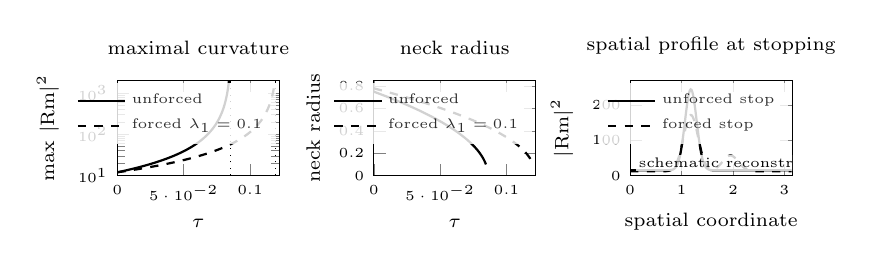
\begin{tikzpicture}[font=\scriptsize]
\begin{groupplot}[
  group style={group size=3 by 1,horizontal sep=1.2cm},
  width=0.30\textwidth,
  height=0.23\textwidth,
  tick label style={font=\tiny},
  label style={font=\scriptsize},
  legend style={font=\tiny,draw=none,fill=white,fill opacity=0.82},
  legend cell align=left,
]
\nextgroupplot[
  title={maximal curvature},
  title style={font=\scriptsize},
  xlabel={$\tau$}, ylabel={max $|\mathrm{Rm}|^2$},
  ymode=log,
  xmin=0,xmax=0.122,
  ymin=10,ymax=2000,
  domain=0:0.0845,
  samples=140,
]
\addplot[thick] {12/(1-x/0.086)^1.35};
\addlegendentry{unforced}
\addplot[thick,dashed,domain=0:0.1185,samples=180] {12/(1-x/0.121)^1.28};
\addlegendentry{forced $\lambda_1=0.1$}
\addplot[black,thin,dotted] coordinates {(0.085,10) (0.085,2000)};
\addplot[black,thin,dotted] coordinates {(0.119,10) (0.119,2000)};

\nextgroupplot[
  title={neck radius},
  title style={font=\scriptsize},
  xlabel={$\tau$}, ylabel={neck radius},
  xmin=0,xmax=0.122,
  ymin=0,ymax=0.85,
  domain=0:0.0845,
  samples=140,
]
\addplot[thick] {0.75*sqrt(max(0,1-x/0.086))};
\addlegendentry{unforced}
\addplot[thick,dashed,domain=0:0.1185,samples=180] {0.75*sqrt(max(0,1-x/0.121))+0.03};
\addlegendentry{forced $\lambda_1=0.1$}

\nextgroupplot[
  title={spatial profile at stopping},
  title style={font=\scriptsize},
  xlabel={spatial coordinate}, ylabel={$|\mathrm{Rm}|^2$},
  xmin=0,xmax=3.15,
  ymin=0,ymax=270,
  domain=0:3.1416,
  samples=180,
]
\addplot[thick] {15+230*exp(-(x-1.18)^2/0.026)};
\addlegendentry{unforced stop}
\addplot[thick,dashed] {12+160*exp(-(x-1.18)^2/0.04)+45*exp(-(x-1.95)^2/0.048)};
\addlegendentry{forced stop}
\node[anchor=south west,fill=white,fill opacity=0.82,text opacity=1,inner sep=1.2pt,font=\tiny] at (rel axis cs:0.03,0.04) {schematic reconstruction};
\end{groupplot}
\end{tikzpicture}
\caption{Ricci--DeTurck flow on warped $S^3$. Left: maximal curvature vs.\ $\tau$. Center: neck radius (zero $=$ pinch). Right: spatial curvature profile at stopping. The engineered forcing $h=2\lambda_1|\Rm|g$ holds the neck open and delays, but does not prevent, the neckpinch.}
\label{fig:dynamics}
\end{figure*}


\begin{corollary}[Net]\label{cor:net}
No forcing in the catalogue---bounded or engineered---is shown to yield a globally curvature-bounded $S^3$ flow.
\end{corollary}

\section{A Planck-barrier invariant region}\label{sec:barrier}

The remaining clean mechanism is not a forcing but a constraint replacing the zero-volume endpoint. Restrict the configuration to a Planck-scale reflecting (no-flux) lower barrier in the base scale.

\begin{theorem}[Invariant region]\label{thm:barrier}
Consider the Berger flow (with any forcing keeping $u\in[\underline u,\bar u]$, $\bar u<\infty$) together with a reflecting barrier at $a=\lP$, i.e.\ the inward drift is projected out whenever $x\le\lP^2$. Then the region $\Omega_{\lP}=\{x\ge\lP^2,\ \underline u\le z/x\le\bar u\}$ is forward-invariant and
\begin{equation}\label{eq:bound}
\sup_{\Omega_{\lP}}|\Rm|^2 \;\le\; \frac{4\,(11\bar u^2+16)}{\lP^4}\;=:\;\frac{C(\bar u)}{\lP^4}.
\end{equation}
\end{theorem}

\begin{proof}
On $\Omega_{\lP}$, $|\Rm|^2=4(16-24u+11u^2)/x^2\le 4(16+11\bar u^2)/\lP^4$ on dropping the negative middle term and using $x\ge\lP^2$. The reflecting condition makes $\{x\ge\lP^2\}$ forward-invariant; bounding $u$ keeps the fibre away from overstretch. A numerical realization with $\lP=0.5$, $\bar u\approx0.15$ gives $\sup|\Rm|^2\cdot\lP^4\approx56$, consistent with $C\le 4(16+11\bar u^2)\approx65$.
\end{proof}

This is the Ricci-flow analogue of the kinematic Kretschmann bound $K\le C/\lP^4$ of compact-$S^3$ minisuperspace, with the no-flux barrier playing the role of the self-adjoint Wheeler--DeWitt endpoint on $L^2([\lP,\infty),a\,da)$ (zero probability flux at $a=\lP$).

\begin{hypothesis}[Boundary correspondence]\label{hyp:wdw}
The reflecting barrier of Theorem~\ref{thm:barrier} corresponds to the self-adjoint Wheeler--DeWitt endpoint of compact minisuperspace. The invariant-region theorem is proved; the cross-framework identification of boundary conditions is a structural conjecture, and the dichotomy ``coercive forcing or no-flux boundary'' is not exhaustive: a third possibility is that the flow is simply incomplete and the Planck endpoint is the physical terminus.
\end{hypothesis}

\section{Numerical methods}\label{sec:numerics}

Berger ODEs~\eqref{eq:odes} (and their forced variants) are integrated with an adaptive stiff solver; the catalogue diagnostics of Table~\ref{tab:contrib} are evaluated symbolically. The warped-$S^3$ flow uses Ricci--DeTurck with round background: writing $g=\varphi^2dx^2+\psi^2 g_{S^2}$ on $x\in[0,\pi]$, the gauge term $\mathcal L_Wg$ with $\bar g=dx^2+\sin^2x\,g_{S^2}$ supplies the $\varphi_{xx}$ diffusion absent from pure Ricci flow, yielding strictly parabolic equations
\begin{align}
\dtau\varphi
&=\tfrac{\varphi_{xx}}{\varphi^2}
 -\tfrac{2\varphi_x^2}{\varphi^3}
 +\tfrac{2\varphi\cos2x}{\psi^2}\nonumber\\
&\quad -\tfrac{2\varphi\sin2x\,\psi_x}{\psi^3}
 +\tfrac{\sin2x\,\varphi_x}{\psi^2}
 +\tfrac{2\psi_x^2}{\varphi\psi^2},\nonumber\\[2pt]
\dtau\psi
&=\tfrac{\psi_{xx}}{\varphi^2}
 -\tfrac1\psi
 -\tfrac{\psi_x^2}{\psi\varphi^2}
 +\tfrac{\sin2x\,\psi_x}{\psi^2}.\nonumber
\end{align}
with pole regularity $\psi(0)=0$, $\varphi(0)=\psi_x(0)$. The singular pole terms cancel analytically at leading order and to machine precision numerically. We verified the round-sphere solution, grid convergence ($N=200\to300$), and the qualitative robustness of the A$'$ relocation result.

\section{Discussion}\label{sec:disc}

The compact-$S^3$ Ricci-type flow makes the coercive curvature problem exactly computable in two solvable families and returns a sharp verdict. The Hopf-fibre channel, attractive as a ``lifted'' compensation, acts on the bounded-curvature direction (Corollary~\ref{cor:directions}); traceless and constant-$\Lambda$ forcing are structurally inert on the singular round mode (Theorem~\ref{thm:nogo}); and the one reduction-level success is a homogeneity artifact that relocates rather than removes the singularity in the genuine inhomogeneous flow (Sec.~\ref{sec:transfer}). What survives is a constraint, not a forcing: a Planck-scale no-flux barrier yields a curvature-bounded invariant region (Theorem~\ref{thm:barrier}).

We emphasize the limitations. All forcing statements are within symmetry reductions; the no-go is sharpest on the round direction, and the transfer failure, while predicted analytically and confirmed dynamically, leaves a sharp, converged conclusion: a three-grid pole-adapted dynamical study shows the canonical engineered term postpones but does not prevent the neckpinch. Whether some more exotic $h[g]$ could control the $\Delta|\Rm|$ source at a neck remains formally open, but the natural curvature-dependent candidate fails, and the regime in which it would have to dominate is stiff and numerically inaccessible to explicit schemes. The boundary correspondence of Hypothesis~\ref{hyp:wdw} is interpretive. No Millennium Problem is advanced; the Poincar\'e conjecture enters only as external justification for the $S^3$ sector.

The honest upshot is a usable formalism: a curvature dictionary, an exact coercive-contribution calculus, a no-go, a transfer-failure mechanism with a validated solver, and a barrier theorem with explicit constant. Negative and conditional though several of its central statements are, each is fully checkable---which is precisely the source of its value.

\section{Programme: quasi-local reconstruction and the universality of the Planck boundary}\label{sec:programme}

This section is interpretive. It proves nothing beyond Secs.~\ref{sec:curv}--\ref{sec:barrier} and is separated from them deliberately: the theorem sections remain dry (Berger, warped $S^3$, no-go, hidden Laplacian source, Planck barrier), while the present section fixes the reading of those results inside the compact-$S^3$ programme. Each principle below is a statement about how the mathematics is to be used, not an additional mathematical claim.

\paragraph*{P1. Quasi-local reconstruction principle.}
The flow parameter $\tau$ in $\dtau g=-2\Ric+h$ is not asserted to be the physical time of the universe. The flow is read as \emph{reconstruction dynamics} on the geometric data $g(\tau)$ of a quasi-local, operationally reconstructible compact domain. Under this reading, the singular limits of Secs.~\ref{sec:curv}--\ref{sec:transfer} mark failures of the chosen reconstruction variables, not necessarily ontological endpoints. What evolves is not ``all of reality'' but the reconstructible domain; when we say the flow shrinks, we say that this domain, under this reconstruction, approaches a boundary regime.

\paragraph*{P2. Local universality of the reconstruction boundary.}
The Planck boundary of Theorem~\ref{thm:barrier} is not tied to one privileged cosmological domain. Any quasi-local compact $S^3$-type domain reconstructed by the same class of geometric and quantum laws encounters the same type of lower boundary, through the mode sequence exhibited by Proposition~\ref{prop:flow}:
\[
\text{shape modes}\;\longrightarrow\;\text{round/trace mode}\;\longrightarrow\;\text{Planck boundary}.
\]
Different domains may have different histories, data, horizons, and embeddings into the larger reality; the reconstruction law assigns the same type of terminal boundary because the local symmetry and scale structure are the same.

\paragraph*{P3. Past and future reconstruction limits are different.}
Backward, the natural boundary of reconstruction is Planckian: the effective configuration space is $a\in[\lP,\infty)$, and $a=0$ is not a state of the effective theory. Forward, the limit is not contraction but loss of operational distinguishability---expansion, dilution, smoothing, horizon formation. The two must not be conflated:
\[
\text{physical expansion}\;\neq\;\text{unnormalized Ricci-flow shrinking}.
\]
They are related only as follows: a physically homogenized late-time domain presents the reconstruction with an almost purely round scale mode (Proposition~\ref{prop:flow}: shape is rounded first), and the unnormalized flow then collapses precisely that remaining mode. ``Shrinking after smoothing'' is therefore an internal signal that the reconstruction variable has exhausted the distinguishable structure of the domain, not a physical prediction of future collapse. In the past the limit is excessive curvature; in the future the limit is insufficient distinguishability. Neither boundary says that reality ends; each says that this language of quasi-local geometric reconstruction ceases to have full meaning there.

\paragraph*{P4. The Hopf lift is a diagnostic, not a rescue.}
Corollary~\ref{cor:directions} is read as follows: the fibre does not save the flow---fibre collapse is the bounded-curvature degeneration---but the lift is valuable as a microscope showing where the singularity is \emph{not}. Quotient descriptions may erase fibre, connection, and holonomy data before one has tested whether they participate in the reconstruction. The Berger family makes the erasure explicit and shows that shape anisotropy is smoothed ($u\to1$) while lifted fibre/connection data are a different type of variable, to be retained or discarded only by explicit modelling choice.

\paragraph*{P5. Boundary over forcing.}
Given Theorem~\ref{thm:nogo} and Sec.~\ref{sec:transfer}---bounded, traceless, fibre-restoring, constant-$\Lambda$, and the engineered curvature-dependent term all failing to control the round mode in the full problem---the Planck no-flux boundary of Theorem~\ref{thm:barrier} is not an ornament. It is the surviving internal candidate for a replacement of surgery on a closed slice, subject to the explicit caveat of Hypothesis~\ref{hyp:wdw} that the dichotomy ``coercive forcing or no-flux boundary'' is not exhaustive.

\paragraph*{P6. Noether-style invariant reading.}
If the variational and geometric structure of the reconstruction law is the same, the associated identities, constraints, and admissible boundary forms are the same~\cite{Noether1918}:
\[
\text{same variational/geometric structure}\;\Longrightarrow\;\text{same identities/constraints/boundary form}.
\]
In this sense the Planck endpoint is an invariant of a class of reconstructions rather than a private feature of one domain. For the boundary module the sharp instance is: a self-adjoint endpoint implies zero probability flux through $a=\lP$, while the minisuperspace wave function $\Psi(\lP)$ may remain finite and nonzero.

\paragraph*{Distinguishability grain.}
The operational content of the lower boundary is a minimal grain of causal distinguishability: below $\lP$ and $t_P=\lP/c$ the effective theory assigns no distinguishable causal-geometric state. The sub-Planck interval is not another physical branch of probability one; it lies outside the assigned operational measure. The region $a<\lP$ does not belong to the effective space of states, so the question of a ``transition'' from it into physical reality does not arise inside this model. Correspondingly, outside the quasi-local domain the theory does not assign an operationally testable geometric state---an epistemic delimitation, not an ontological claim of absence.

\paragraph*{Axis of the programme.}
\begin{quote}
\emph{The Planck boundary is not the beginning of the universe; it is the universal lower boundary of quasi-local geometric reconstruction.}
\end{quote}
The chain established by this line of work is: compact $S^3$ topology $\to$ Ricci-type curvature criterion $\to$ Hopf/$SU(2)$ diagnostic split $\to$ no-go for natural forcing $\to$ Planck-barrier invariant region $\to$ self-adjoint Wheeler--DeWitt endpoint $\to$ open bridge to quantum-gravity-like boundary structure. None of these principles adds to what is proved; each fixes what the proofs are for.

\section*{Reproducibility}
All curvature identities were verified by independent symbolic computation; the DeTurck solver and diagnostic scripts are available with the manuscript.

\appendix

\section{Convention and curvature derivation}\label{app:conv}
With $[e_i,e_j]=\lambda\,\epsilon_{ijk}e_k$ the Koszul formula gives, on the diagonal left-invariant metric $g=\mathrm{diag}(A,B,C)$,
\[
\Ric_{11}=\frac{\lambda^2}{2}\frac{A^2-(B-C)^2}{BC}\quad\text{(cyclic)} ,
\]
so the round value $A=B=C=1$ is $\Ric_{ii}=\lambda^2/2$; demanding $\Ric=2g$ fixes $\lambda=2$. Specializing $A=B=x$, $C=z$ yields Proposition~\ref{prop:curv}. The identity $|\Rm|^2=4|\Ric|^2-R^2$ holds in dimension three because the Weyl tensor vanishes, providing an independent check; a direct contraction of the Riemann tensor built from the same connection gives a third. The unforced ODEs~\eqref{eq:odes} follow from $\dot g_{ii}=-2\Ric_{ii}$ in the coframe, and $\dot u=8u(1-u)/x$ from the quotient rule; $u=1$ is the unique stable fixed point.

\section{Coercive contributions via homogeneity}\label{app:euler}
$|\Rm|^2$ is homogeneous of degree $-2$ in $(x,z)$, so $(x\partial_x+z\partial_z)|\Rm|^2=-2|\Rm|^2$. A conformal forcing $(P,Q)=(2\Lambda x,2\Lambda z)$ contributes $2\Lambda(x\partial_x+z\partial_z)|\Rm|^2=-4\Lambda|\Rm|^2$; with $\Lambda=\lambda_1|\Rm|$ this is $-4\lambda_1|\Rm|^3$. The fibre term $(0,\mu)$ contributes $\mu\,\partial_z|\Rm|^2=8\mu(11z-12x)/x^4$; the trace-free term ($h_{33}=-\tfrac{2z}{x}h_{11}$) contributes $-32h_{11}(x-z)(4x-11z)/x^5$, vanishing at $z=x$. These are the entries of Table~\ref{tab:contrib} and the content of Theorem~\ref{thm:nogo}.

\section{Verification log}\label{app:verify}
Every dimensionful identity below was produced and checked in computer algebra (SymPy) or by convergent numerics:
the $\lambda=2$ normalization; $\Ric,R,|\Ric|^2,|\Rm|^2$ and the three-way cross-check; the sectional curvatures; the unforced ODEs, $\dot u$, and the volume law $\tfrac{d}{d\tau}\ln V=-R$; the round reaction constant $C_3^{\mathrm B}=4/\sqrt3$; the exact forcing contributions $-4\Lambda|\Rm|^2$, $-4\lambda_1|\Rm|^3$, the fibre sign-flip at $u=12/11$, and the traceless vanishing at $u=1$; the bounded-curvature collapse $|\Rm|^2\to64/a^4$; the warped-$S^3$ curvature and the conformal variation $\delta R=-2\varphi R-4\Delta\varphi$; the Ricci--DeTurck round-sphere solution to machine accuracy; and the three-grid (uniform $N=200,300$; pole-clustered) convergence of the forced neckpinch at $\lambda_1=0.1$ to $\tau\approx0.119$.

\begin{thebibliography}{9}
\bibitem{Hamilton1982} R.~S.~Hamilton, \emph{Three-manifolds with positive Ricci curvature}, J.\ Diff.\ Geom.\ \textbf{17}, 255 (1982).
\bibitem{ChowKnopf} B.~Chow and D.~Knopf, \emph{The Ricci Flow: An Introduction}, AMS (2004).
\bibitem{Perelman1} G.~Perelman, \emph{The entropy formula for the Ricci flow and its geometric applications}, arXiv:math/0211159 (2002).
\bibitem{Perelman2} G.~Perelman, \emph{Ricci flow with surgery on three-manifolds}, arXiv:math/0303109 (2003).
\bibitem{MorganTian} J.~Morgan and G.~Tian, \emph{Ricci Flow and the Poincar\'e Conjecture}, AMS/Clay (2007).
\bibitem{AngenentKnopf} S.~Angenent and D.~Knopf, \emph{An example of neckpinching for Ricci flow on $S^{n+1}$}, Math.\ Res.\ Lett.\ \textbf{11}, 493 (2004).
\bibitem{Noether1918} E.~Noether, \emph{Invariante Variationsprobleme}, Nachr.\ Ges.\ Wiss.\ G\"ottingen, 235 (1918).
\end{thebibliography}


\end{document}
